% !TeX root = ../Thesis.tex

%************************************************
\chapter{Evaluation}\label{ch:evaluation}
%************************************************
\glsresetall % Resets all acronyms to not used

To answer the main question of this thesis, whether the integration of \glspl{NN} into \gls{VPR} can improve its performance, we optimize and thoroughly evaluate our system.

\section{Evaluation Scenario}

First describing our method of evaluation as well as the specific settings used, we then evaluate the various \gls{NN} candidates against each other to determine the best network structure. Following this, the original \gls{VPR} Placer is evaluated and compared with our versions integrating \glspl{NN}.

\subsection{Selected Benchmarks}\label{ch:benchmarks}

For the final evaluation, we select three circuits from the \gls{VPR} benchmark suite that were not used in any prior part of this project, namely \textit{mcml.blif}, \textit{or1200.blif}, and \textit{diffeq2.blif}. These circuits are selected quasi-randomly from the \textit{small} circuits of the \gls{VTR} benchmark suite. The reasons for this choice are limited resources for the evaluation as well as a performance issue detailed in Section \ref{ch:Justification}.

In the same manner, we also select an \textit{evaluation} set of one circuit (\textit{raygentop.blif}), which will be needed for our chosen method of model selection, detailed in Section \ref{ch:model-selection}. This set is intentionally small to keep the computational effort of model selection manageable.

As the \gls{VPR} Placement algorithm is a pseudo-randomized heuristic not guaranteed to yield reproducible results (when starting from a different state), each evaluation on each of this circuits will be performed with 3 redundant placing attempts with different random seeds to ensure robust results. 

Finally, the median of the three performance scores is chosen rather than the mean, which makes our evaluation robust against outliers.

\subsection{Runtime/Quality Trade-off}

Our metric of choice is runtime/quality trade-off, specifically discretely sampled routing quality (minimum channel width and critical path length) for certain approximate absolute placement runtimes. These runtimes, or sampling points, are selected per benchmark circuit relative to the runtime of the unchanged \gls{VPR} Placer (t\textsubscript{p}) as:

\begin{itemize}
	\item 1   * t\textsubscript{p}, or \textit{sampling point 1}
	\item 10  * t\textsubscript{p}, or \textit{sampling point 10}
	\item 50  * t\textsubscript{p}, or \textit{sampling point 50}
	\item 250 * t\textsubscript{p}, or \textit{sampling point 250}
	\item 1250 * t\textsubscript{p}, or \textit{sampling point 1250}
\end{itemize}

The actual runtime, while not A-Priori \textit{predictable} for a certain configuration of the modified \gls{VPR} Placer, can easily be \textit{controlled} with the \textit{inner\_num} setting of \gls{VPR}.\cite{vtr8} 

Based on observations we state without formal proof that most of the computations of the \gls{VPR} Placer are performed inside each of these steps. Furthermore, while steps perform random actions and can have vastly differing runtime, within a certain \textit{temperature level} steps with different runtimes are distributed randomly, and the number of steps per temperature is generally high. Therefore, changing this number of steps will not change the distribution of step runtimes within a certain temperature-level, which means their average runtime remains approximately the same. Therefore, changes to the \textit{inner\_num} parameter, which is a linear factor for the actual number of steps performed, affect the total runtime of the modified \gls{VPR} Placer approximately linearly.

By placing a benchmark circuit using a fixed setting for \textit{inner\_num}, the runtime at this setting is acquired. As early experiments showed that the runtime of the \gls{VPR} Placer using \glspl{NN} is one to two orders of magnitude slower than using \gls{HPWL}, this value is set to $0.01*num\_blocks^(4/3)$, which equals one-hundredth of the default value of the \gls{VPR} Placer. Therefore, this first check is estimated to take approximately as much time as the unchanged \gls{VPR} at sampling point 1.

Now, \textit{inner\_num} can be scaled appropriately to gain quality scores at each sampling point.

Evaluating the performance of a certain \gls{NN} during model selection consists of the following steps:

\begin{itemize}
	\item integration into \gls{VPR}
	\item determining the runtime over \textit{inner\_num}
	\item setting \textit{inner\_num} appropriately for sampling point 10
	\item placing the evaluation circuit three times
	\item routing each placement and logging median quality 
\end{itemize}

The final evaluation of the best \gls{CNN} and \gls{RNN} against unchanged \gls{VPR} is performed as follows:

\begin{itemize}
	\item integration into \gls{VPR}
	\item determining the runtime over \textit{inner\_num}
	\item setting \textit{inner\_num} appropriately for sampling point 1
	\item placing the test circuits three times
	\item routing each placement and logging median quality per circuit
	\item repeating for the remaining sampling points
\end{itemize}

The thus computed quality/runtime trade-off is then compared with that of the unchanged \gls{VPR} Placer.

The \gls{VPR} Router primarily optimizes the \textit{channel width}, or maximum number of parallel routing channels used by the routing, by determining the minimum routable value via binary search. Therefore we select \textit{channel width} as the primary evaluation metric. In the final evaluation, we will, however, also compare critical path lengths, as this, being \gls{VPR}'s secondary optimization target, defines the maximum operable frequency of the circuit, directly influencing its computational capabilities.

\section{Model Selection}\label{ch:model-selection}

Although \glspl{NN} automatically tune their parameters to fit the target function, the structure and properties of the network itself has to be specified explicitly. While recent works try to automate even this, it is usually still necessary to manually design networks to achieve good results.

During model selection, \glspl{CNN} and \glspl{RNN} are evaluated independently from each other and using the same methodology. This yields a choice for the best \gls{CNN} and the best \gls{RNN}, which will both again be integrated into \gls{VPR} and evaluated against the unchanged Placer.  

\subsection{Empirical Model Search}

Typically, a first working design is found empirically through experimentation, based largely on best practices, related works, and intuition. In this case, the strict requirements on the runtime of the networks restricted the search space considerably, and the model candidates described in Chapters \ref{ch:cnn-design} and \ref{ch:rnn-design} represent the obvious choices for small and simple networks.

From these candidates, the best one is selected by evaluating each independently on evaluation data different from the training and the final test data, and comparing the results.

\subsection{\gls{HPO}}

\begin{figure}
	\begin{subfigure}[b]{0.49\linewidth}
		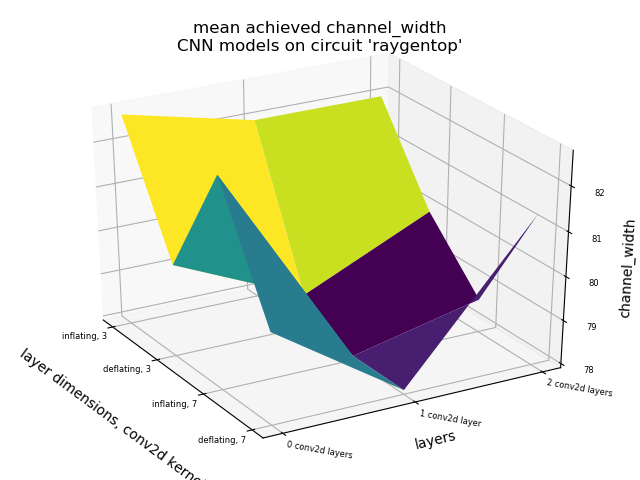
\includegraphics[width=\linewidth]{plots/cnn-hyperopt-chan-width.png}
		\caption{\glspl{CNN} - channel width}
	\end{subfigure}
	\begin{subfigure}[b]{0.49\linewidth}
		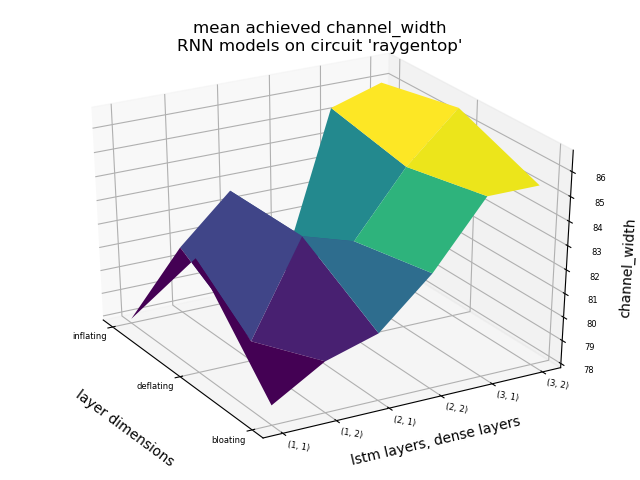
\includegraphics[width=\linewidth]{plots/rnn-hyperopt-chan-width.png}
		\caption{\glspl{RNN} - channel width}
	\end{subfigure}
	\begin{subfigure}[b]{0.49\linewidth}
		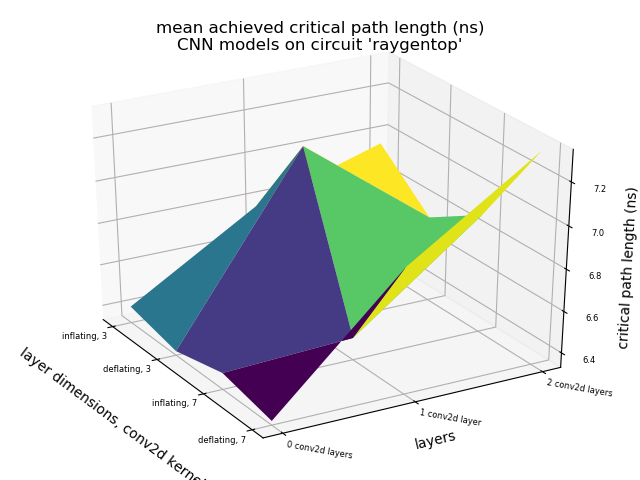
\includegraphics[width=\linewidth]{plots/cnn-hyperopt-critical-path.png}
		\caption{\glspl{CNN} - critical path length}
	\end{subfigure}
	\begin{subfigure}[b]{0.49\linewidth}
		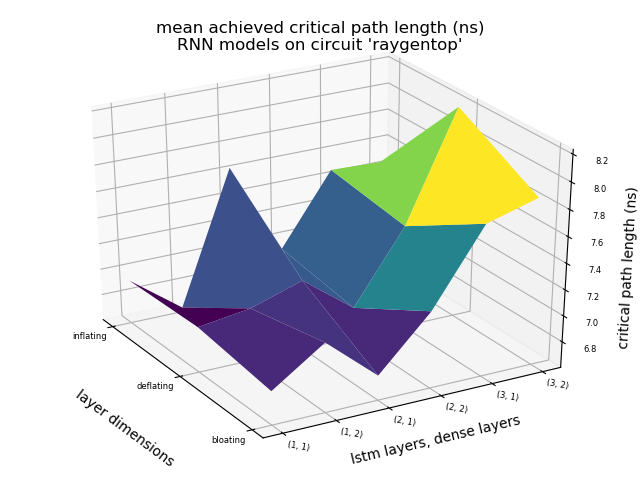
\includegraphics[width=\linewidth]{plots/rnn-hyperopt-critical-path.png}
		\caption{\glspl{RNN} - critical path length}
	\end{subfigure}
	\caption{Achieved performance over model configurations.}
	\label{fig:eval-hyperopt-surface}
\end{figure}

As these groups of candidates are generated from discrete parameters, e.g. dense layer count, this model selection approach constitutes a grid search over these hyperparameters.

By evaluating the \gls{NN} candidates on the evaluation set at sampling point 10 we determine their relative performance. A visualization of the results in Figure \ref{fig:eval-hyperopt-surface} clearly shows a correlation between network complexity and routing quality: Smaller networks produce better results, with the exception of \glspl{CNN} without convolutional layers. These models, using less time for a prediction, allow for a higher number of moves per temperature step, although producing less accurate predictions than their more complex counterparts. The properties of convolutional layers, while computationally being rather expensive (at least compared to the "tiny" dense layers), seem to be beneficial to accurately predict the wiring cost. As the \gls{LSTM} layers of the \glspl{RNN} are required to encode the input data for the following dense layers, their suitedness to the problem can not be measured that easily.

\begin{table}
	\resizebox{\textwidth}{!}{
	\begin{tabular}{lllrr}
		\toprule
		&           &   &  channel\_width &  critical\_path \\
		conv\_layer & structure & kernel &                &                   \\
		count &  & size &                &                   \\
		\midrule
		0 & deflating & -1 &           80.0 &           6.27 \\
		& inflating & -1 &           80.0 &           6.26 \\
		1 & deflating & 3 &           78.0 &           7.21 \\
		&           & 7 &           78.0 &           6.66 \\
		& inflating & 3 &           82.0 &           6.58 \\
		&           & 7 &           78.0 &           6.12 \\
		2 & deflating & 3 &           80.0 &           6.61 \\
		&           & 7 &           80.0 &           7.22 \\
		& inflating & 3 &           80.0 &           7.14 \\
		&           & 7 &           78.0 &           6.81 \\
		\bottomrule
	\end{tabular}
	}
	\caption{Results of \gls{CNN} HPO. Median of reached scores for each model variant.}
	\label{table:cnn-hyperopt-results}
\end{table}

\begin{table}
	\resizebox{\textwidth}{!}{
	\begin{tabular}{lllrr}
		\toprule
		&   &           &  channel\_width &  critical\_path \\
		lstm\_layer & dense\_layer & structure &                &                   \\
		count & count &  &                &                   \\
		\midrule
		1 & 1 & bloating &           78.0 &              6.83 \\
		&   & deflating &           80.0 &              6.82 \\
		&   & inflating &           78.0 &              7.03 \\
		& 2 & bloating &           80.0 &              7.47 \\
		&   & deflating &           78.0 &              6.83 \\
		&   & inflating &           80.0 &              6.56 \\
		2 & 1 & bloating &           80.0 &              6.82 \\
		&   & deflating &           82.0 &              7.14 \\
		&   & inflating &           82.0 &              7.50 \\
		& 2 & bloating &           84.0 &              7.06 \\
		&   & deflating &           82.0 &              6.97 \\
		&   & inflating &           78.0 &              6.95 \\
		3 & 1 & bloating &           84.0 &              7.44 \\
		&   & deflating &           84.0 &              7.40 \\
		&   & inflating &           86.0 &              7.47 \\
		& 2 & bloating &           86.0 &              7.70 \\
		&   & deflating &           86.0 &              7.44 \\
		&   & inflating &           86.0 &              7.69 \\
		\bottomrule
	\end{tabular}
	}
	\caption{Results of \gls{RNN} HPO. Median of reached scores for each model variant.}
	\label{table:rnn-hyperopt-results}
\end{table}

The exact results are presented in Table \ref{table:cnn-hyperopt-results} and Table \ref{table:rnn-hyperopt-results} (for information about the performance at each individual placement attempt see Appendix \ref{ch:AdditionalData}). We thus select \textit{1\_conv\_layers\_deflating\_kernel\_size\_7} and \textit{1\_lstm\_layers\_1\_dense\_layers\_inflating} as the best \gls{CNN} and \gls{RNN} models, respectively. 

Note that these choices might not be obvious. Indeed, also factoring in the achieved critical path length, these are not the best models with respect to median performance. However, as we decided to only consider channel width for the \gls{HPO}, the critical path length was not considered at this point. Instead, average (mean) and best (minimum) performance on channel width were used to resolve ties.

\begin{figure}
	\begin{subfigure}[b]{0.49\linewidth}
		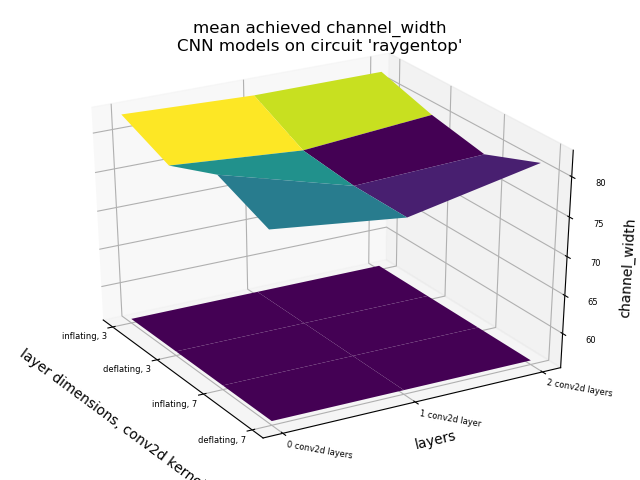
\includegraphics[width=\linewidth]{plots/cnn-hyperopt-chan-width-with-reference.png}
		\caption{\glspl{CNN} - channel width}
	\end{subfigure}
	\begin{subfigure}[b]{0.49\linewidth}
		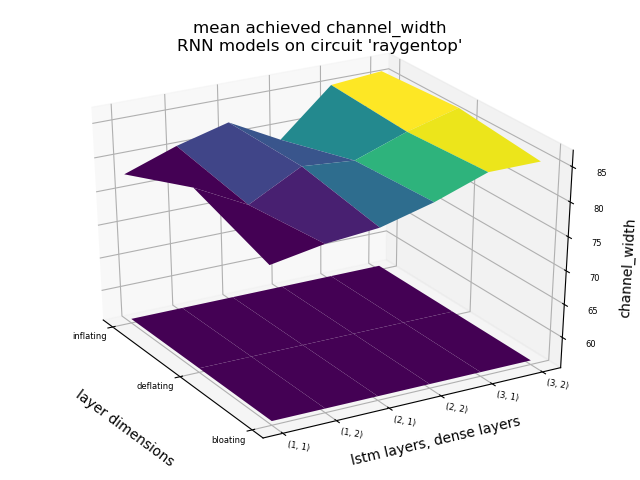
\includegraphics[width=\linewidth]{plots/rnn-hyperopt-chan-width-with-reference.png}
		\caption{\glspl{RNN} - channel width}
	\end{subfigure}
	\begin{subfigure}[b]{0.49\linewidth}
		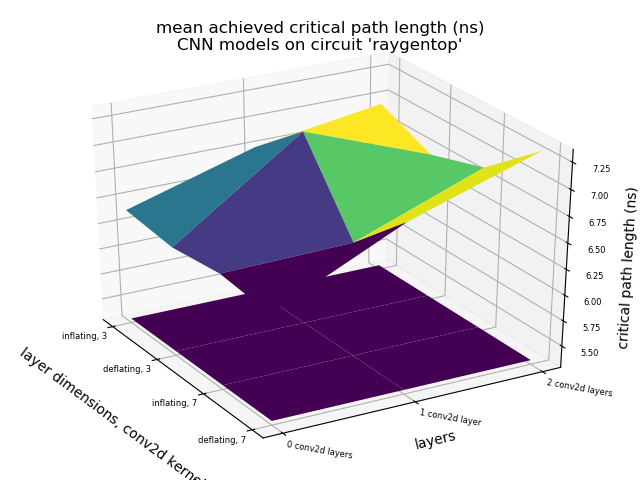
\includegraphics[width=\linewidth]{plots/cnn-hyperopt-critical-path-with-reference.png}
		\caption{\glspl{CNN} - critical path length}
	\end{subfigure}
	\begin{subfigure}[b]{0.49\linewidth}
		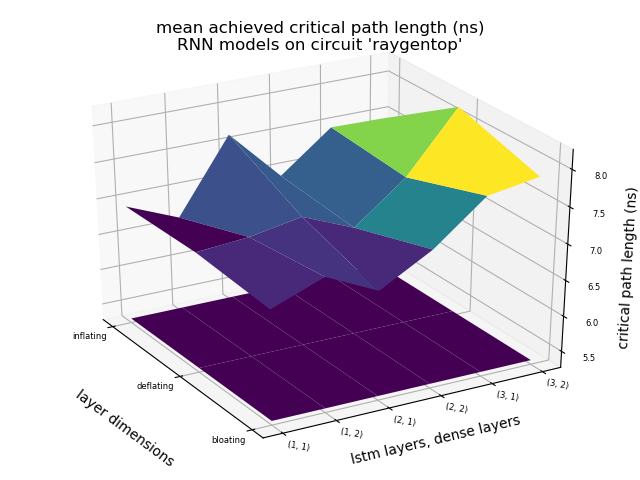
\includegraphics[width=\linewidth]{plots/rnn-hyperopt-critical-path-with-reference.png}
		\caption{\glspl{RNN} - critical path length}
	\end{subfigure}
	\caption{Achieved performance over model configurations with performance of reference system.}
	\label{fig:eval-hyperopt-surface-reference}
\end{figure}

By comparing the performance to that of the unchanged \gls{VPR} Placer we can, however, see that none of the \glspl{NN} is able to beat \gls{HPWL} at sampling point 10 (see Figure \ref{fig:eval-hyperopt-surface-reference}).

\section{Results}

With a single network per type, the modified \gls{VPR} Placer can now be evaluated against the unchanged version (reference system).

\begin{figure}
	\centering
	\begin{subfigure}[b]{0.49\linewidth}
		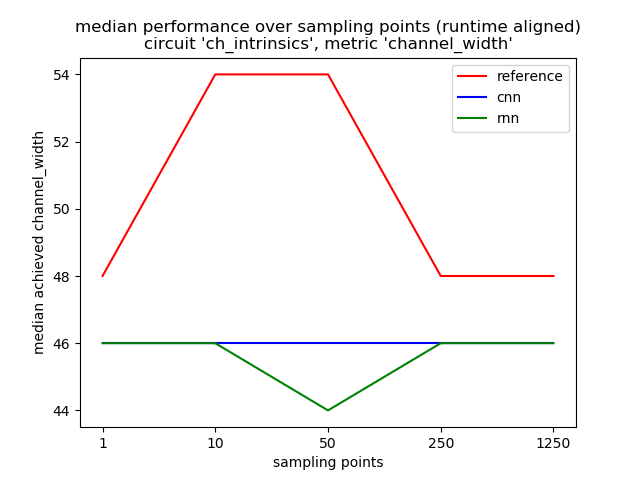
\includegraphics[width=\linewidth]{plots/eval-ch_intrinsics-chan-width-median-full.png}
	\end{subfigure}
	\begin{subfigure}[b]{0.49\linewidth}
		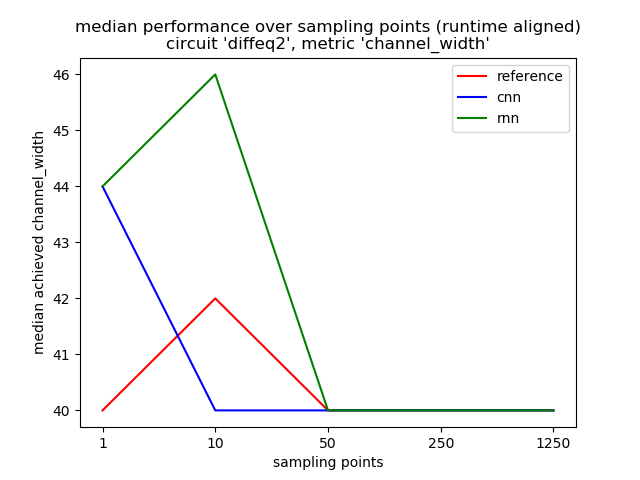
\includegraphics[width=\linewidth]{plots/eval-diffeq2-chan-width-median-full.png}
	\end{subfigure}
	\begin{subfigure}[b]{0.49\linewidth}
		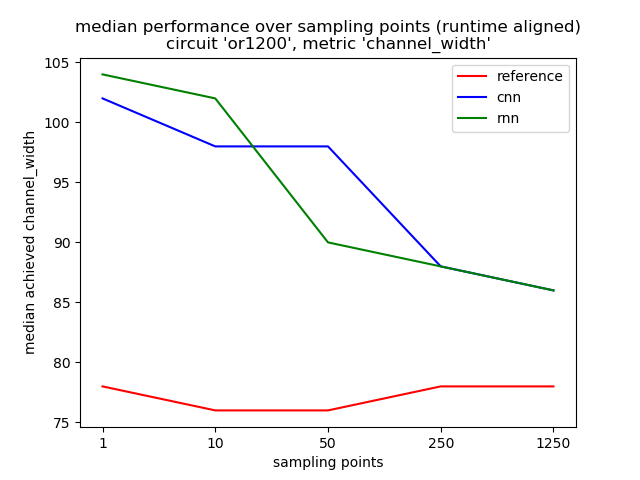
\includegraphics[width=\linewidth]{plots/eval-or1200-chan-width-median-full.png}
	\end{subfigure}
	\begin{subfigure}[b]{0.49\linewidth}
		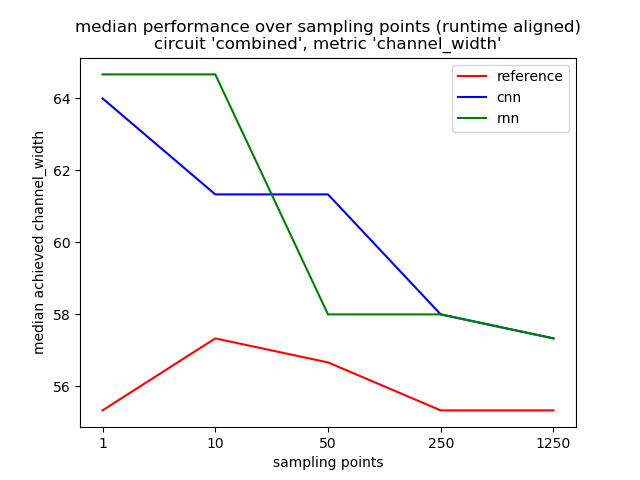
\includegraphics[width=\linewidth]{plots/eval-combined-chan-width-median-full.png}
	\end{subfigure}
	\caption{Median of achieved channel width over sampling points per circuit.}
	\label{fig:eval-chan-width-median}
\end{figure}

Figure \ref{fig:eval-chan-width-median} shows the achieved channel widths for the reference system and our \gls{CNN} and \gls{RNN} versions on the test set. Our modified placer using \glspl{NN} is able to significantly outperform the reference system on one of the small circuits and manages to match it on the other (top), but is inferior on the larger one (bottom left). 

When combining the results on all three circuits with equal weights, the reference system has higher performance overall. However, even being able to perform better on \textit{some} circuits can be seen as an improvement, as placing with both the modified and the reference system and individually selecting the better result is also a viable option.

\begin{figure}
	\centering
	\begin{subfigure}[b]{0.49\linewidth}
		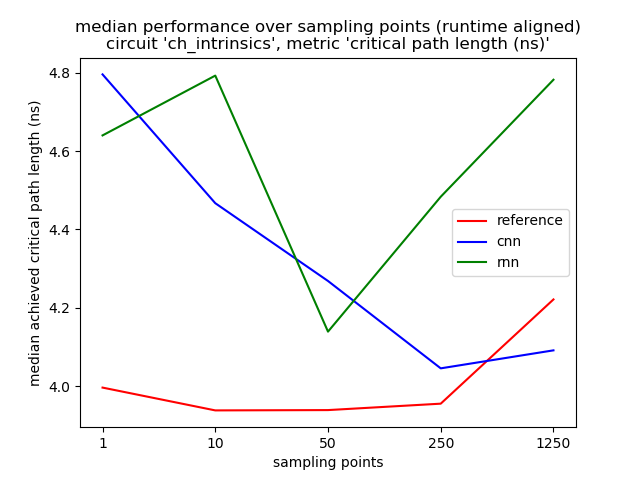
\includegraphics[width=\linewidth]{plots/eval-ch_intrinsics-critical-path-median-full.png}
	\end{subfigure}
	\begin{subfigure}[b]{0.49\linewidth}
		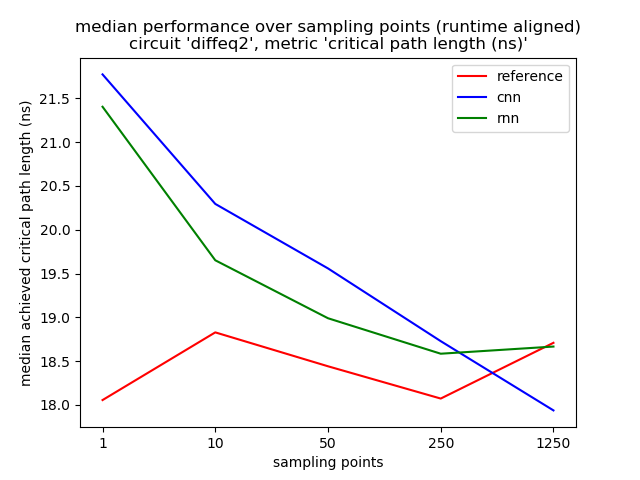
\includegraphics[width=\linewidth]{plots/eval-diffeq2-critical-path-median-full.png}
	\end{subfigure}
	\begin{subfigure}[b]{0.49\linewidth}
		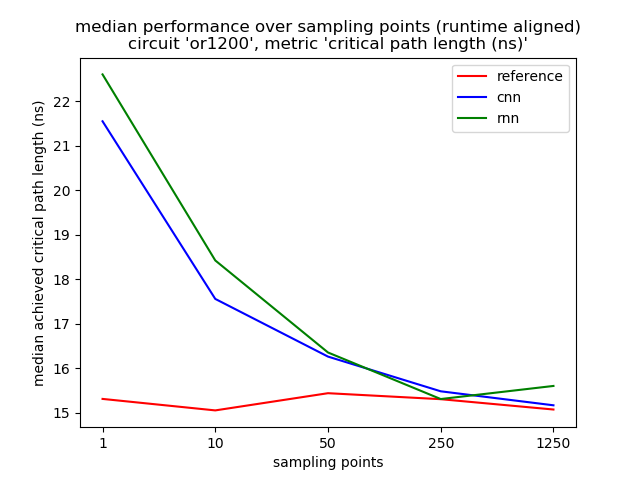
\includegraphics[width=\linewidth]{plots/eval-or1200-critical-path-median-full.png}
	\end{subfigure}
	\begin{subfigure}[b]{0.49\linewidth}
		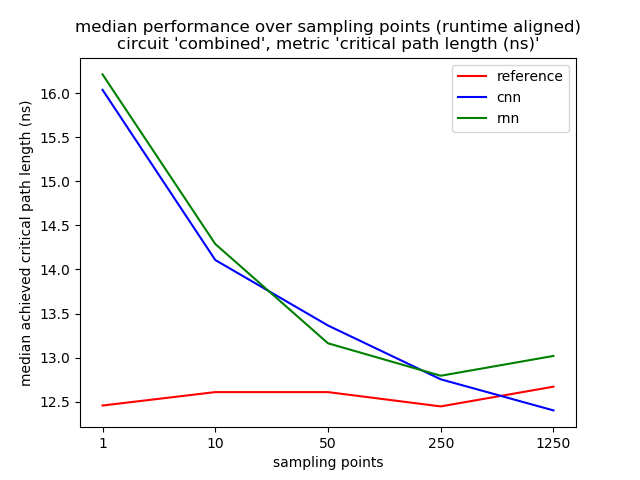
\includegraphics[width=\linewidth]{plots/eval-combined-critical-path-median-full.png}
	\end{subfigure}
	\caption{Median of achieved critical path length over sampling points per circuit.}
	\label{fig:eval-critical-path-median}
\end{figure}

What's more, the quality/runtime trade-offs of both our modified systems show a significant downward trend. While this is not that clearly visible in the achieved channel widths on both smaller circuits, it is very pronounced in the critical path delays shown in Figure \ref{fig:eval-critical-path-median}. This could imply its performance relative to the reference system might increase further beyond the domain we evaluated, i.e. for larger sampling points. However, the quasi-logarithmic scale of the x-axes of these Figures might make this trend seem steeper than it is.

Equivalent Figures showing mean and minimum instead of median can be found in the Appendix \ref{ch:AdditionalData}.

One can also observe that while the \gls{CNN} version initially always beats the \gls{RNN} version, the performance difference clearly diminishes on higher sampling points. The \gls{RNN} version, however, seems less stable than the \gls{CNN} version, which consistently shows a smooth curve. Therefore, we would declare \glspl{CNN} to be the superior approach based on the available data, but \glspl{RNN} should not be excluded from further evaluations until stronger evidence is available.

Our modified systems exhibit a significantly steeper downward slope than the reference system. Therefore, we believe them to be able to outperform the reference system consistently at even higher sampling points than those evaluated in this work. However, the practical usability of our modified systems in their current state is questionable. They only manage to beat the reference system at very high sampling points and for small circuits. While performance on large circuits is not sufficiently evaluated due to lack of resources, large sampling points are impractical due to their high runtime. Sampling point 1250 implies a 1250-fold runtime than the reference system takes at standard settings. While this might be acceptable on small benchmarks and toy circuits, it seems infeasible on realistically sized problems.

\begin{table}
\resizebox{\textwidth}{!}{
\begin{tabular}{lllrrrrrrrr}
	\toprule
	&    & metric & \multicolumn{4}{l}{channel\_width} & \multicolumn{4}{l}{critical\_path} \\
	&    & attempt &             1 &      2 &      3 &     mean &             1 &      2 &      3 &    mean \\
	circuit & sampling & type &               &        &        &         &               &        &        &        \\
		    & point	   & 	  &               &        &        &         &               &        &        &        \\
	\midrule
	diffeq2 & 1    & reference &          \textbf{40.0} &   40.0 &   40.0 &   40.00 &         18.35 &  18.00 &  \textbf{18.05} &  18.14 \\
	&      & rnn &          40.0 &   46.0 &   \textbf{44.0} &   43.33 &         21.73 &  21.24 &  \textbf{21.40} &  21.46 \\
	&      & cnn &          \textbf{44.0} &   44.0 &   42.0 &   43.33 &         20.08 &  \textbf{21.77} &  21.98 &  21.28 \\
	& 10   & reference &          56.0 &   38.0 &   \textbf{42.0} &   45.33 &         \textbf{18.83} &  18.98 &  18.51 &  18.77 \\
	&      & rnn &          40.0 &   \textbf{46.0} &   46.0 &   44.00 &         20.40 &  \textbf{19.65} &  19.46 &  19.83 \\
	&      & cnn &          \textbf{42.0} &   40.0 &   38.0 &   40.00 &         21.14 &  \textbf{20.30} &  19.90 &  20.44 \\
	& 50   & reference &          \textbf{40.0} &   40.0 &   42.0 &   40.67 &         18.60 &  18.13 &  \textbf{18.44} &  18.39 \\
	&      & rnn &          46.0 &   \textbf{40.0} &   40.0 &   42.00 &         20.23 &  \textbf{18.99} &  18.17 &  19.13 \\
	&      & cnn &          \textbf{40.0} &   40.0 &   38.0 &   39.33 &         19.48 &  \textbf{19.56} &  19.68 &  19.57 \\
	& 250  & reference &          44.0 &   38.0 &   \textbf{40.0} &   40.67 &         17.72 &  19.36 &  \textbf{18.07} &  18.39 \\
	&      & rnn &          \textbf{40.0} &   46.0 &   38.0 &   41.33 &         \textbf{18.58} &  17.78 &  19.03 &  18.47 \\
	&      & cnn &          38.0 &   \textbf{40.0} &   40.0 &   39.33 &         18.75 &  18.45 &  \textbf{18.73} &  18.64 \\
	& 1250 & reference &          \textbf{40.0} &   44.0 &   40.0 &   41.33 &         \textbf{18.71} &  19.18 &  18.60 &  18.83 \\
	&      & rnn &          \textbf{40.0} &   40.0 &   38.0 &   39.33 &         \textbf{18.67} &  18.59 &  18.81 &  18.69 \\
	&      & cnn &          \textbf{40.0} &   40.0 &   40.0 &   40.00 &         \textbf{17.94} &  18.37 &  17.74 &  18.02 \\
	or1200 & 1    & reference &          76.0 &   \textbf{78.0} &   78.0 &   77.33 &         \textbf{15.32} &  15.50 &  15.18 &  15.33 \\
	&      & rnn &         \textbf{104.0} &  106.0 &  104.0 &  104.67 &         \textbf{22.60} &  22.55 &  23.07 &  22.74 \\
	&      & cnn &         106.0 &  \textbf{102.0} &  102.0 &  103.33 &         20.87 &  23.50 &  \textbf{21.55} &  21.97 \\
	& 10   & reference &          \textbf{76.0} &   80.0 &   76.0 &   77.33 &         \textbf{15.06} &  14.92 &  15.20 &  15.06 \\
	&      & rnn &         106.0 &  100.0 &  \textbf{102.0} &  102.67 &         19.46 &  \textbf{18.42} &  17.82 &  18.57 \\
	&      & cnn &          94.0 &   \textbf{98.0} &  100.0 &   97.33 &         18.28 &  17.07 &  \textbf{17.56} &  17.64 \\
	& 50   & reference &          \textbf{76.0} &   78.0 &   74.0 &   76.00 &         \textbf{15.44} &  15.22 &  15.63 &  15.43 \\
	&      & rnn &          98.0 &   \textbf{90.0} &   90.0 &   92.67 &         17.16 &  16.34 &  \textbf{16.36} &  16.62 \\
	&      & cnn &          \textbf{98.0} &   94.0 &  100.0 &   97.33 &         \textbf{16.27} &  16.39 &  16.17 &  16.27 \\
	& 250  & reference &          \textbf{78.0} &   76.0 &   78.0 &   77.33 &         15.89 &  14.79 &  \textbf{15.31} &  15.33 \\
	&      & rnn &          82.0 &   \textbf{88.0} &   88.0 &   86.00 &         15.35 &  15.22 &  \textbf{15.31} &  15.29 \\
	&      & cnn &          \textbf{88.0} &   88.0 &   92.0 &   89.33 &         15.33 &  \textbf{15.49} &  15.49 &  15.44 \\
	& 1250 & reference &          \textbf{78.0} &   78.0 &   74.0 &   76.67 &         15.64 &  \textbf{15.08} &  15.07 &  15.26 \\
	&      & rnn &          \textbf{86.0} &   88.0 &   86.0 &   86.67 &         14.90 &  15.90 &  \textbf{15.61} &  15.47 \\
	&      & cnn &          \textbf{86.0} &   86.0 &   88.0 &   86.67 &         \textbf{15.17} &  15.04 &  15.61 &  15.27 \\
	ch\_intrinsics & 1    & reference &          54.0 &   \textbf{48.0} &   46.0 &   49.33 &          3.94 &   \textbf{4.00} &   4.64 &   4.19 \\
	&      & rnn &          \textbf{46.0} &   46.0 &   48.0 &   46.67 &          4.24 &   5.88 &   \textbf{4.64} &   4.92 \\
	&      & cnn &          \textbf{46.0} &   46.0 &   48.0 &   46.67 &          4.24 &   4.98 &   \textbf{4.80} &   4.67 \\
	& 10   & reference &          \textbf{54.0} &   54.0 &   54.0 &   54.00 &          \textbf{3.94} &   3.94 &   4.39 &   4.09 \\
	&      & rnn &          \textbf{46.0} &   46.0 &   44.0 &   45.33 &          4.18 &   \textbf{4.79} &   4.79 &   4.59 \\
	&      & cnn &          \textbf{46.0} &   44.0 &   46.0 &   45.33 &          \textbf{4.47} &   4.71 &   4.38 &   4.52 \\
	& 50   & reference &          \textbf{54.0} &   54.0 &   48.0 &   52.00 &          \textbf{3.94} &   4.04 &   3.90 &   3.96 \\
	&      & rnn &          46.0 &   \textbf{44.0} &   44.0 &   44.67 &          4.00 &   \textbf{4.14} &   4.18 &   4.11 \\
	&      & cnn &          \textbf{46.0} &   44.0 &   46.0 &   45.33 &          4.23 &   4.65 &   \textbf{4.27} &   4.38 \\
	& 250  & reference &          \textbf{48.0} &   44.0 &   54.0 &   48.67 &          \textbf{3.96} &   4.42 &   3.91 &   4.10 \\
	&      & rnn &          44.0 &   \textbf{46.0} &   50.0 &   46.67 &          4.59 &   \textbf{4.48} &   4.05 &   4.37 \\
	&      & cnn &          \textbf{46.0} &   44.0 &   46.0 &   45.33 &          4.03 &   4.28 &   \textbf{4.05} &   4.12 \\
	& 1250 & reference &          \textbf{48.0} &   48.0 &   48.0 &   48.00 &          6.01 &   3.89 &   \textbf{4.22} &   4.71 \\
	&      & rnn &          44.0 &   48.0 &  \textbf{46.0} &   46.00 &          5.37 &   4.55 &   \textbf{4.78} &   4.90 \\
	&      & cnn &          50.0 &   \textbf{46.0} &   46.0 &   47.33 &          \textbf{4.09} &   5.02 &   3.92 &   4.35 \\
	\bottomrule
\end{tabular}
}
\caption{Complete summary of evaluation results. Median for each mode, circuit, and sampling point marked in \textbf{bold}.}
\label{table:eval-complete}
\end{table}

The complete results of the evaluation are listed in Table \ref{table:eval-complete}.

\subsection{Justification}\label{ch:Justification}

Of course, an approximation of the runtime/quality trade-off using only three rather small circuits is far from perfect, and a more thorough evaluation is needed to make any profound claims. This, however, does not fall in the scope of this work for two reasons. Firstly, the subject of this work was to implement a prototype and evaluate the general feasibility of this approach. Secondly, the evaluation is computationally highly intensive, and evaluating circuits of a higher order of magnitude quickly becomes unfeasible on commodity hardware.

Regarding the first reason, both goals of this thesis have been fulfilled. We provided a working prototype implementing in-placement wirelength estimation in the \gls{VPR} Placer using either \glspl{CNN} or \glspl{RNN}, and showed that it is indeed possible for this approach to outperform the traditional one using the \gls{HPWL} heuristic.

\subsubsection{Issues}

Furthermore, while evaluation on our selected test set and sampling points completes within the scale of several hours to one day, we noticed a disproportionate increase in runtime for larger circuits. While the time needed for placing the circuit matched our expectations (based on the formula for computing the number of moves per temperature level), for some reason it becomes nearly impossible to route large circuits placed with the modified placer. A single routing step, which is performed in the manner of seconds when routing a placement produced by the reference system, reaches runtimes of more than an hour on a placement produced by our \gls{NN} based approach. 

\begin{figure}
	\begin{subfigure}[b]{0.49\linewidth}
		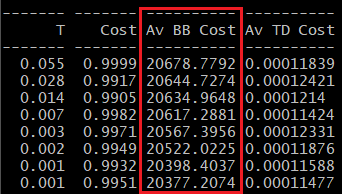
\includegraphics[width=\linewidth]{plots/log_place_ref.png}
	\end{subfigure}
	\hfill
	\begin{subfigure}[b]{0.49\linewidth}
		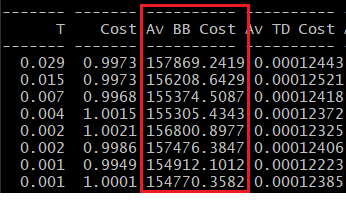
\includegraphics[width=\linewidth]{plots/log_place_cnn.png}
	\end{subfigure}
	\begin{subfigure}[b]{0.49\linewidth}
		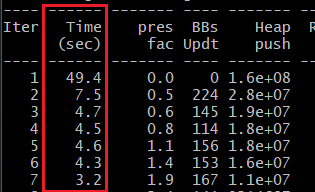
\includegraphics[width=\linewidth]{plots/log_route_ref.png}
		\caption{Reference System}
	\end{subfigure}
	\hfill
	\begin{subfigure}[b]{0.49\linewidth}
		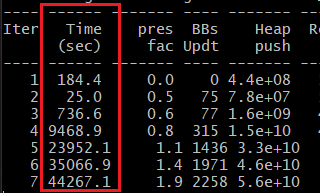
\includegraphics[width=\linewidth]{plots/log_route_cnn.png}
		\caption{\gls{CNN} Version}
	\end{subfigure}
	\caption{Partial Placement (top) and Routing (bottom) logs for circuit \textit{mcml.blif}. Normal behaviour on reference system (left), increased \textit{\gls{BB} cost} and routing time on \gls{CNN} version (right).}
	\label{fig:eval-problem-logs}
\end{figure}

\subsubsection{Possible Reasons}

We further noticed a substantial increase of reported \textit{average \gls{BB} cost}, or average estimated wirelength, during placement (see Figure \ref{fig:eval-problem-logs}). This roughly tenfold increase might originate from the different target values of the used wire length estimators. Pure \gls{HPWL} is a lower bound to the actual wiring cost, and even the corrected/scaled \gls{HPWL} used in \gls{VPR} can be assumed to generally underestimate large nets. As our \glspl{NN} try to predict the actual wirelength and might make errors in both directions, a certain increase in average placement driven cost is not surprising.

Still, an increase of this magnitude might also be caused by some bug or incompatible code, although we were not able to find any evidence of this when inspecting the \gls{VPR} source code.

This change in the general scale of the \gls{BB} cost could also have incurred other implications. In the simulated annealing algorithm that constitutes the core of the \gls{VPR} Placer timing and placement driven costs are combined to assess the effects of a move. Therefore the weighting of the components of this combination might be required to mitigate this effect.

However, seeing as the simulated annealer still converges as in the unchanged system, those effects should not be too strong. The eventual decrease in estimated \gls{BB} cost of the temporary placement matches that of the reference system.

This issue was only noticed in the final phase of this work when large circuits were placed with the modified placer and subsequently routed for the first time. Therefore, we were only able to perform basic tests and analysis.

\subsection{Future Work}

As such, it is left as future work to identify and solve this issue. Once this is done, the system can be re-evaluated on a larger test set also containing very large circuits. 

If this system is evaluated further, it would also be appropriate to raise the number of redundant placements, which would allow for quantifying one's confidence in in the evaluation results, as Xu et al. do in \cite{star-plus-paper}.

Apart from that, it might prove worthwhile to profile the modified system and check for performance bottlenecks. Especially the \gls{tf} interface seems overly complicated for such a simple network, and for using only online prediction. Therefore, optimising the integration of the \gls{NN} might reduce the complexity of this runtime critical part of the system.

Last but not least, optimising the \glspl{NN} themselves could also yield further improvements.
